\documentclass[a4paper]{article}
\usepackage{fullpage} % Smaller margins
\usepackage{graphicx}
\graphicspath{{./images}}

%% Document Header
\title{Weebapedia (working title)}
\author{Alice Charatonik}
\date{}

\begin{document}
\maketitle

\section{Introduction}
An encyclopedia-like database of anime information, moreso focused on answering questions than showing the user all possibly relevant information.

\section{Objectives}
Make it easy for any user to find information about their favorite anime shows or characters, as well as the people and teams who worked on those shows or characters.
\begin{itemize}
  \item Broad questions: eg. "What is Attack on Titan?" or "Who was Satoshi Kon?"
  \item Narrow questions: eg. "Who did Satoshi Kon work with most frequently?"
  \item Relationship questions: eg. "Has Hideaki Anno worked with anyone who would go on to work on Attack on Titan?"
\end{itemize}

\section{Prior Art}
\subsection{MyAnimeList}
\includegraphics[width=\textwidth]{MAL.png}
\subsection{AniList}
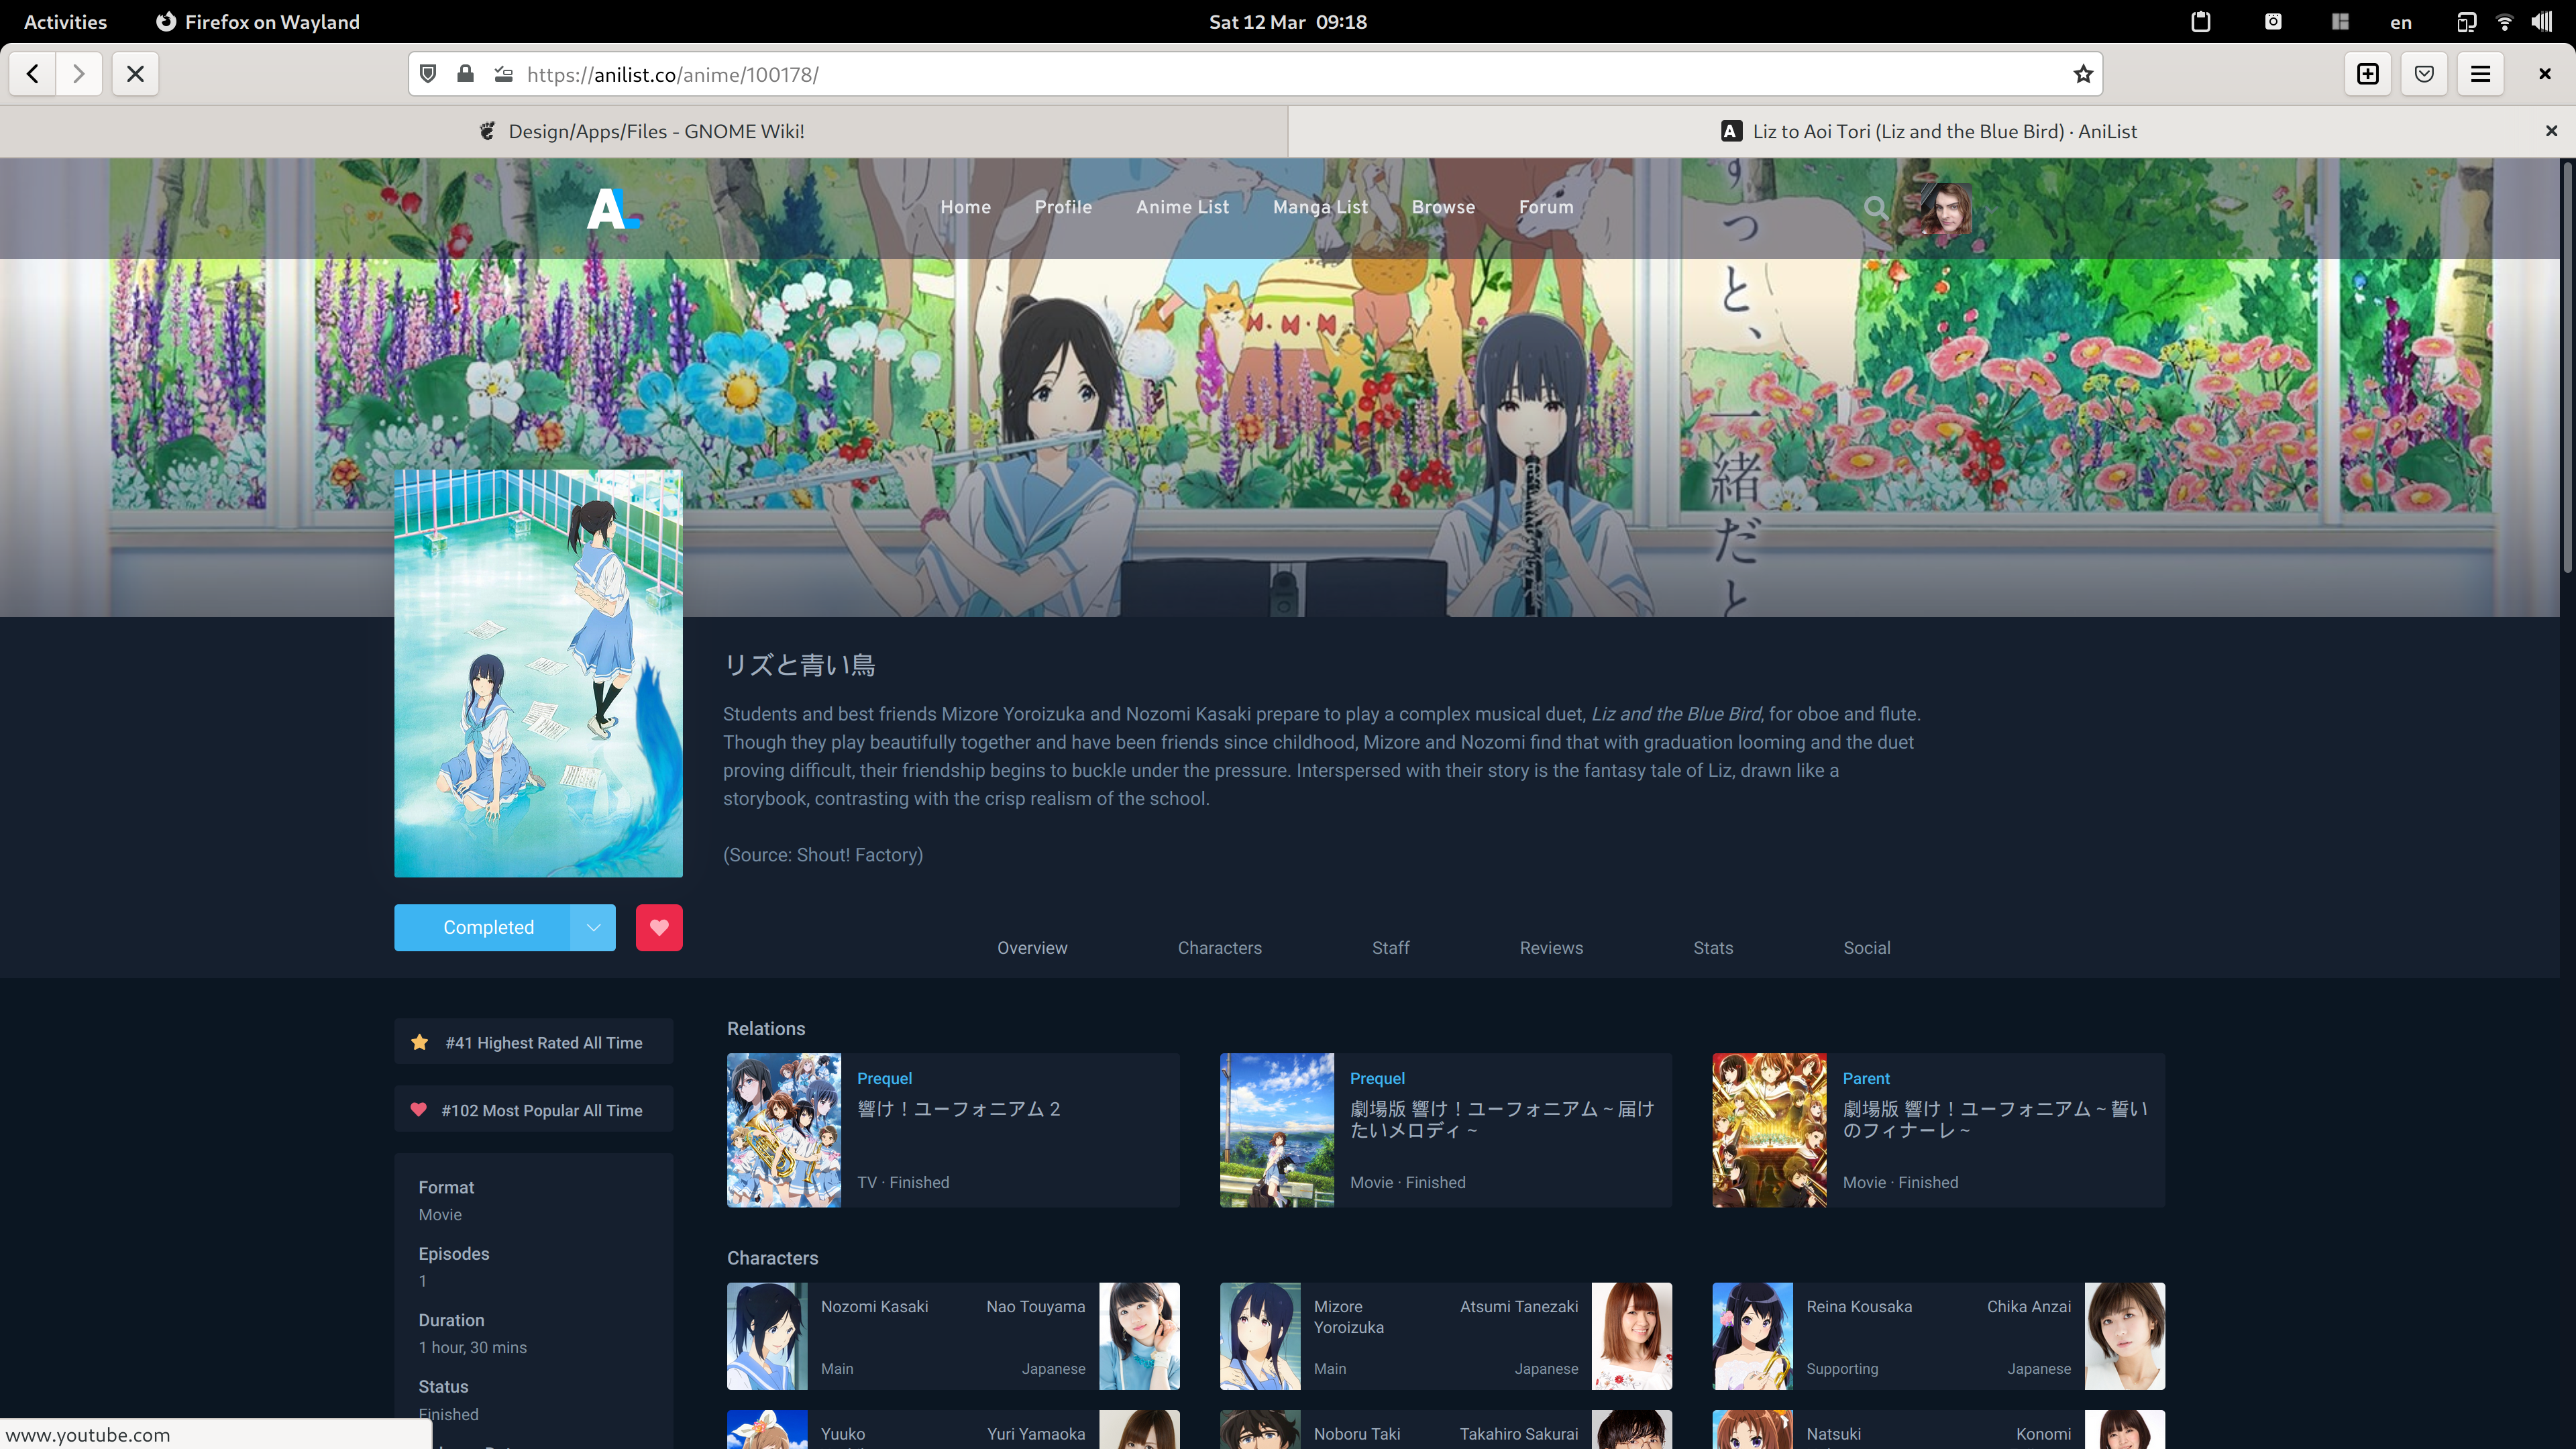
\includegraphics[width=\textwidth]{aniList.png}
\subsection{Kitsu}
\includegraphics[width=\textwidth]{Kitsu.png}
\subsection{Anime Planet}
\includegraphics[width=\textwidth]{AP.png}
\subsection{AniDB}
\includegraphics[width=\textwidth]{aniDB.png}

\section{Considerations}
\begin{itemize}
  \item Most competition is focused on community-created content. Favorites, ratings, reviews, etc. We consider these out of scope.
  \item Most also have a focusing on list-making or cataloging. Eg. "What anime have you seen, what anime have I seen?" This too, is out of scope. Our primary goal is a focus on ease of research.
  \item Most do not make it easy to make claims about the relationships between different anime. For example, if you make a claim like "Studio Trigger is mostly composed of ex-Gainax employees," there is no easy way to look this up. 
  \item Making the above easy is what differentiates our product.
\end{itemize}

\end{document}